\lab{Introduction to Plotting: Matplotlib and Mayavi}{Matplotlib and Mayavi}
\objective{Data visualization is a key component of scientific computing.
Python has several standard packages that work in conjunction with NumPy and SciPy to visualize data contained in arrays.
In this lab we introduce Matplotlib, the most commonly-used visualization library in Python.
We also introduce Mayavi, a module with extensive 3-D visualization capabilities.
These plotting techniques will be used in the majority of the labs in this curriculum.}
\label{lab:Matplotlib_and_Mayavi}


\section*{Line Plots} % =======================================================

The quickest way to visualize a simple 1-D array is via a \emph{line plot}.
In the following example, we create an array to visualize and plot it using the \li{matplotlib} module.\footnote{Like NumPy and SciPy, Matplotlib is \emph{not} part of the Python standard library, but is included in most Python distributions.}

\begin{lstlisting}
>>> import numpy as np
>>> from matplotlib import pyplot as plt

>>> y = np.array([n**2 for n in xrange(-5, 6)])
>>> y
array([25, 16,  9,  4,  1,  0,  1,  4,  9, 16, 25])

# Visualize the plot.
>>> plt.plot(y)                     # Draw the line plot.
<<[<matplotlib.lines.Line2D object at 0x1084762d0>]>>
>>> plt.show()                      # Reveal the resulting plot.
\end{lstlisting}

The result is shown in Figure \ref{fig:basic1}.
Just as \li{np} is a standard alias for NumPy, \li{plt} is a standard alias for \li{matplotlib.pyplot} in the Python community.

The call \li{plt.plot(y)} creates a figure and draws straight lines connecting the entries of \li{y} relative to the $y$-axis.
The $x$-axis is by default the index of the array, namely the integers from $0$ to $10$.
Calling \li{plt.show()} then displays the figure.

\begin{figure}[H] % plt.plot(y) compared to plt.plot(x,y).
\captionsetup[subfigure]{justification=centering}
\centering
\begin{subfigure}{.5\textwidth}
    \centering
    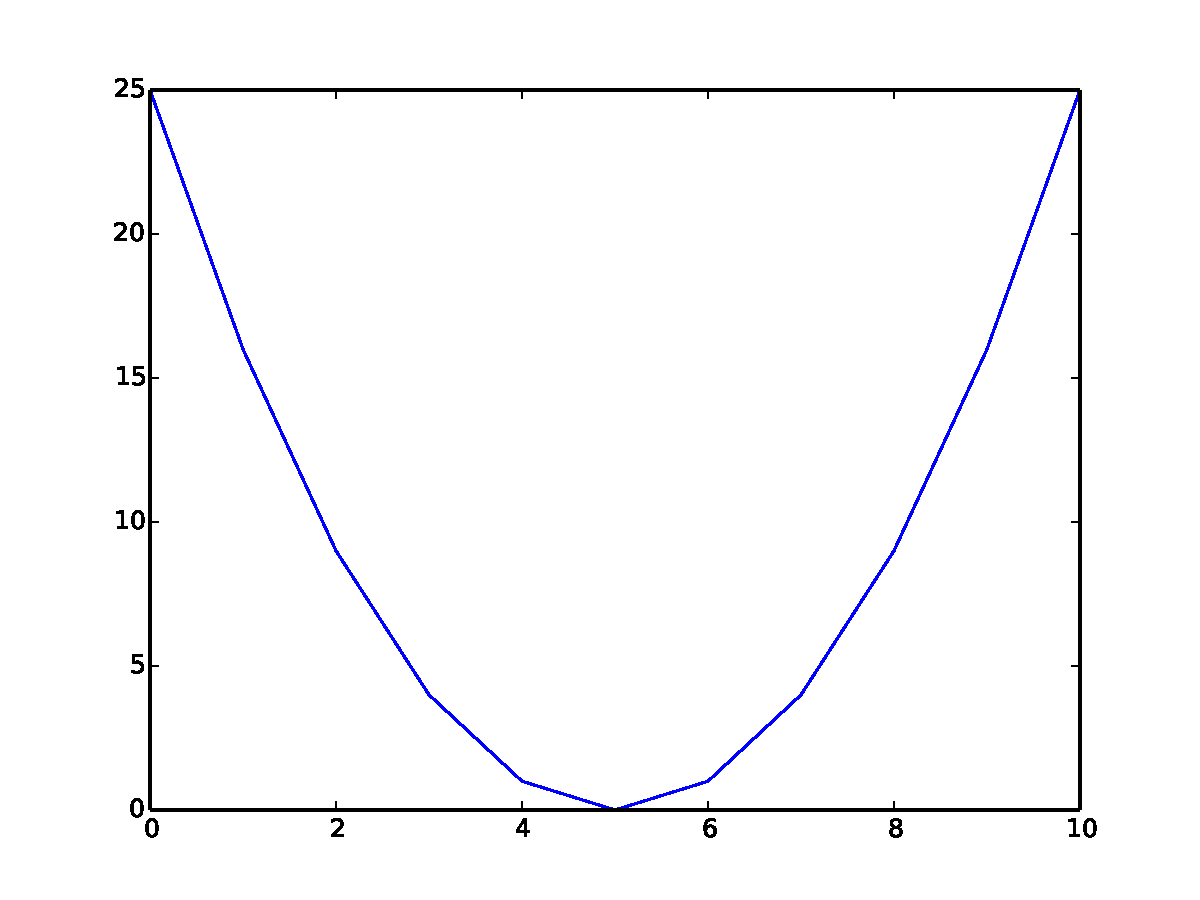
\includegraphics[width=\linewidth]{basic1.pdf}
    \caption{\li{plt.plot(y)} uses the indices of\\the array for the $x$-axis.}
    \label{fig:basic1}
\end{subfigure}%
\begin{subfigure}{.5\textwidth}
    \centering
    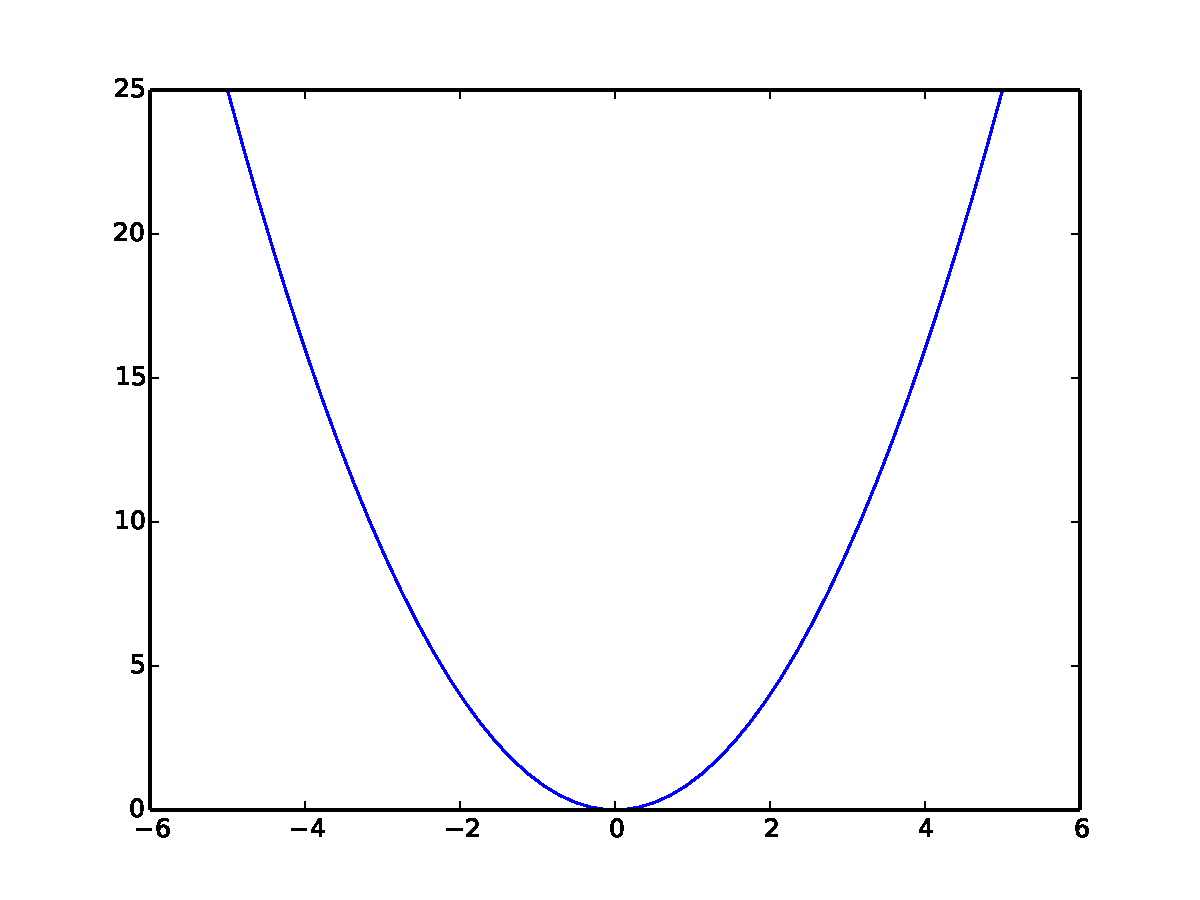
\includegraphics[width=\linewidth]{basic2.pdf}
    \caption{\li{plt.plot(x,y)} specifies both the\\domain and the range.}
    \label{fig:basic2}
\end{subfigure}
\caption{Simple plots of $f(x) = x^2$ over the interval $x\in[-5,5]$.}
\end{figure}

\begin{problem} % Law of Large Numbers / NumPy review.
Write a function that accepts an integer $n$ as input.
\begin{enumerate}
\item Use \li{np.random.randn()} or \li{np.random.normal()} to create an $n\times n$ array of values randomly sampled from the standard normal distribution.
\item Compute the mean of each row of the array.
\\(Hint: use \li{np.mean()} and specify the \li{axis} keyword argument.)
\item Return the variance of these means (this should be a single scalar).
\end{enumerate}
Define a new function that creates an array of the results of the first function with inputs $n = 100,\ 200,\ \ldots,\ 1000$.
% \begin{lstlisting}
% >>> y = np.array([prob1(n) for n in xrange(100,1100,100)])
% \end{lstlisting}
%
Plot (and show) the resulting array.

This illustrates one version of the \emph{Law of Large Numbers}, which will be discussed later on in Volume II.
\end{problem}

\subsection*{Specifying a Domain} % -----------------------------------------

An obvious problem with Figure \ref{fig:basic1} is that the $x$-axis does not correspond correctly to the $y$-axis for the function $f(x) = x^2$ that is being drawn.
To correct this, we provide an array for the domain as well as one for the range.
That is, we first define an array \li{x} for the domain, then use that array to calculate the range \li{y} of the function we would like to plot.
The command \li{plt.plot(x,y)} then plots \li{x} against \li{y}.
Both arrays must have the same number of elements to be compatible.

Another problem with Figure \ref{fig:basic1} is its poor resolution; the curve is visibly bumpy, especially near the bottom of the curve.
NumPy's \li{np.linspace()} function makes it easy to get a higher-resolution domain.
Recall that \li{range()} and \li{np.arange()} return a list or array of evenly-spaced values in a given interval, where the \emph{spacing} between the entries is specified.
In contrast, \li{np.linspace()} creates an array of evenly-spaced values in a given interval where the \emph{number of elements} is specified.

\begin{lstlisting}
# 4 evenly-spaced values between 0 and 32 (including endpoints).
>>> np.linspace(0, 32, 4) 
array([  0.        ,  10.66666667,  21.33333333,  32.        ])

# Get 50 evenly-spaced values from -5 to 5 (including endpoints).
>>> x = np.linspace(-5, 5, 50)
>>> y = x**2                        # Calculate the range of f(x) = x**2.
>>> plt.plot(x, y)
>>> plt.show()
\end{lstlisting}

The resulting plot is shown in Figure \ref{fig:basic2}.
Note that this time, the $x$-axis is correctly aligned with the $y$-axis.
The resolution is also much better because \li{x} and \li{y} have $50$ entries each instead of only $10$.

All calls to \li{plt} functions modify the same figure until \li{plt.show()} is executed, which displays the current figure and resets the system.
The next time a \li{plt} function is called a new figure is created.
This makes it possible to plot several lines in a single figure.

\begin{comment} % Wordy details and unnecessary plots for multi-line plotting.
We can take advantage of this system to plot multiple lines on the same axes.
For example, the following code plots ten lines, each with random values at integers from 1 to 10. 
The output is in Figure \ref{fig:statemachine}.

\begin{lstlisting}
x = np.linspace(1, 10, 10)

# Create a 10x10 array of uniformly distributed values in [0,1).
y = np.random.rand(10, 10)

# Plot each row of y
for row in y:
    plt.plot(x, row)
plt.show()
\end{lstlisting}

Alternatively, we can produce the same graph with a single call to \li{plt.plot()}.

\begin{lstlisting}
plt.plot(x, y[0], x, y[1], x, y[2], x, y[3], x, y[4], x, y[5], x, y[6], x, y[7], x, y[8], x, y[9])
plt.show()
\end{lstlisting}
\end{comment}

\begin{problem} % Plot two lines (sin() and cos()).
Plot the functions $\sin(x)$, $\cos(x)$, and $\arctan(x)$ on the domain $[-2\pi, 2\pi]$ (use \li{np.pi} for $\pi$).
% Call \li{plt.xlim(-2*np.pi, 2*np.pi)} before \li{plt.show()} to stretch the $x$-axis appropriately.
Make sure the domain is refined enough to produce a figure with good resolution.
\end{problem}

\begin{info} % Interactive Mode.
Plotting can seem a little mystical because the actual plot doesn't appear until \li{plt.show()} is executed.
Matplotlib's \emph{interactive mode}, particularly useful in IPython, allows the user to see the plot be constructed one piece at a time.
Use \li{plt.ion()} to turn interactive mode on and \li{plt.ioff()} to turn it off.
This is very useful for customizing a plot on the fly.

Try executing the following commands in IPython:

\begin{lstlisting}
In [1]: import numpy as np
In [2]: from matplotlib import pyplot as plt

# Turn interactive mode on and make some plots.
In [3]: plt.ion()
In [4]: x = np.linspace(1, 4, 100)
In [5]: plt.plot(x, np.log(x))
In [6]: plt.plot(x, np.exp(x))

# Clear the figure, then turn interactive mode off.
In [7]: plt.clf()
In [8]: plt.ioff()
\end{lstlisting}

It is wise to use interactive mode \textbf{only} with IPython, as it exhibits erratic behavior when producing subplots or multiple figures.
\end{info}

\section*{Plot Customization} % ===============================================

\li{plt.plot()} receives several keyword arguments for customizing the drawing.
For example, the color and style of the line are specified by the following string arguments.

\begin{table}[H] % Color and style.
\begin{tabular}{r|l}
    Code & Color \\
    \hline
    \li{'b'} & blue\\
    \li{'g'} & green\\
    \li{'r'} & red\\
    \li{'c'} & cyan\\
    \li{'m'} & magenta\\
    % \li{'y'} & yellow\\
    \li{'k'} & black\\
    % \li{'w'} & white
\end{tabular}
\qquad
\begin{tabular}{r|l}
    Code & Style \\
    \hline
    \li{'-'}' & solid line\\
    \li{'--'} & dashed line\\
    \li{'-.'} & dash-dot line\\
    \li{':'} & dotted line\\
    % \li{'.'} & point marker\\
    \li{'o'} & circle marker\\
    % \li{'*'} & star marker\\
    \li{'+'} & plus marker
\end{tabular}
% \caption{Common colors and line styles. See Appendix \ref{mpltables} for more.}
\end{table}

Specify one or both of these string codes as an argument to \li{plt.plot()} to change from the default color and style.
Other \li{plt} functions further customize a figure.

\begin{table}[H]
\centering
\begin{tabular}{r|l}
    Function & Description\\
    \hline
    % \li{grid()} & Add grid lines\\
    \li{legend()} & Place a legend in the plot\\
    % \li{text()} & Add text at a given position on the plot\\
    \li{title()} & Add a title to the plot\\
    \li{xlim()} & Set the limits of the $x$-axis\\
    \li{ylim()} & Set the limits of the $y$-axis\\
    % \li{xticks()} & set the location of the tick marks on the x axis, returns current locations if no arguments are given\\
    % \li{yticks()} & set the location of the tick marks on the y axis, returns current locations if no arguments are given\\
    \li{xlabel()} & Add a label to the $x$-axis\\
    \li{ylabel()} & Add a label to the $y$-axis
\end{tabular}
\end{table}

\begin{lstlisting}
>>> x1 = np.linspace(-2, 4, 100)
>>> plt.plot(x1, np.exp(x1), 'g:', linewidth=2, label="Exponential")
>>> plt.title("This is the title.")
>>> plt.legend(loc="upper left")    # plt.legend() uses the 'label' argument of
>>> plt.show()                      # plt.plot() to create a legend.

>>> x2 = np.linspace(1, 4, 100)
>>> plt.plot(x2, np.log(x2), 'r+', linewidth=2)
>>> plt.xlim(0, 5)                  # Set the visible limits of the x axis.
>>> plt.xlabel("The x axis")        # Give the x axis a label.
>>> plt.show()
\end{lstlisting}

\begin{figure}[H] % Figure customizations.
\captionsetup[subfigure]{justification=centering}
\centering
\begin{subfigure}{.5\textwidth}
    \centering
    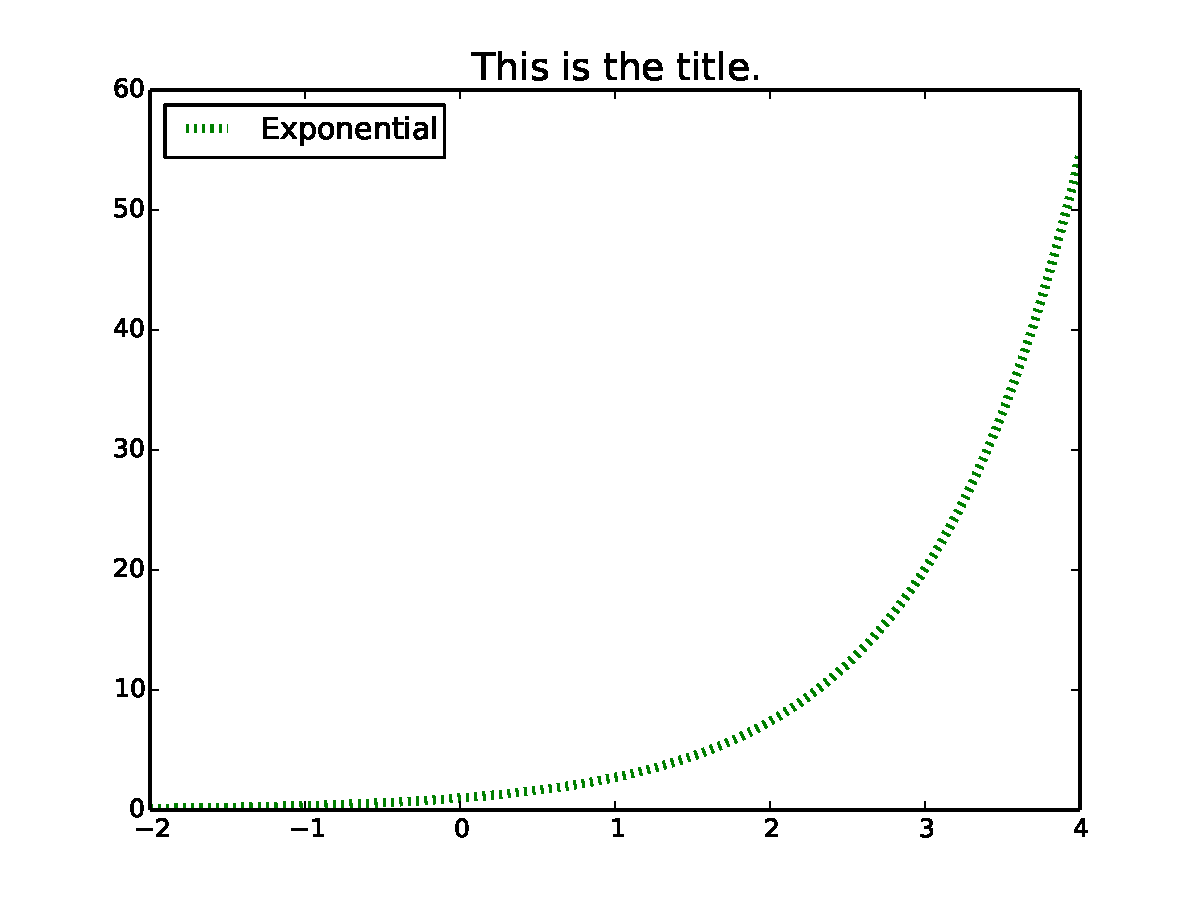
\includegraphics[width=\linewidth]{custom1.pdf}
    \label{fig:custom1}
\end{subfigure}%
\begin{subfigure}{.5\textwidth}
    \centering
    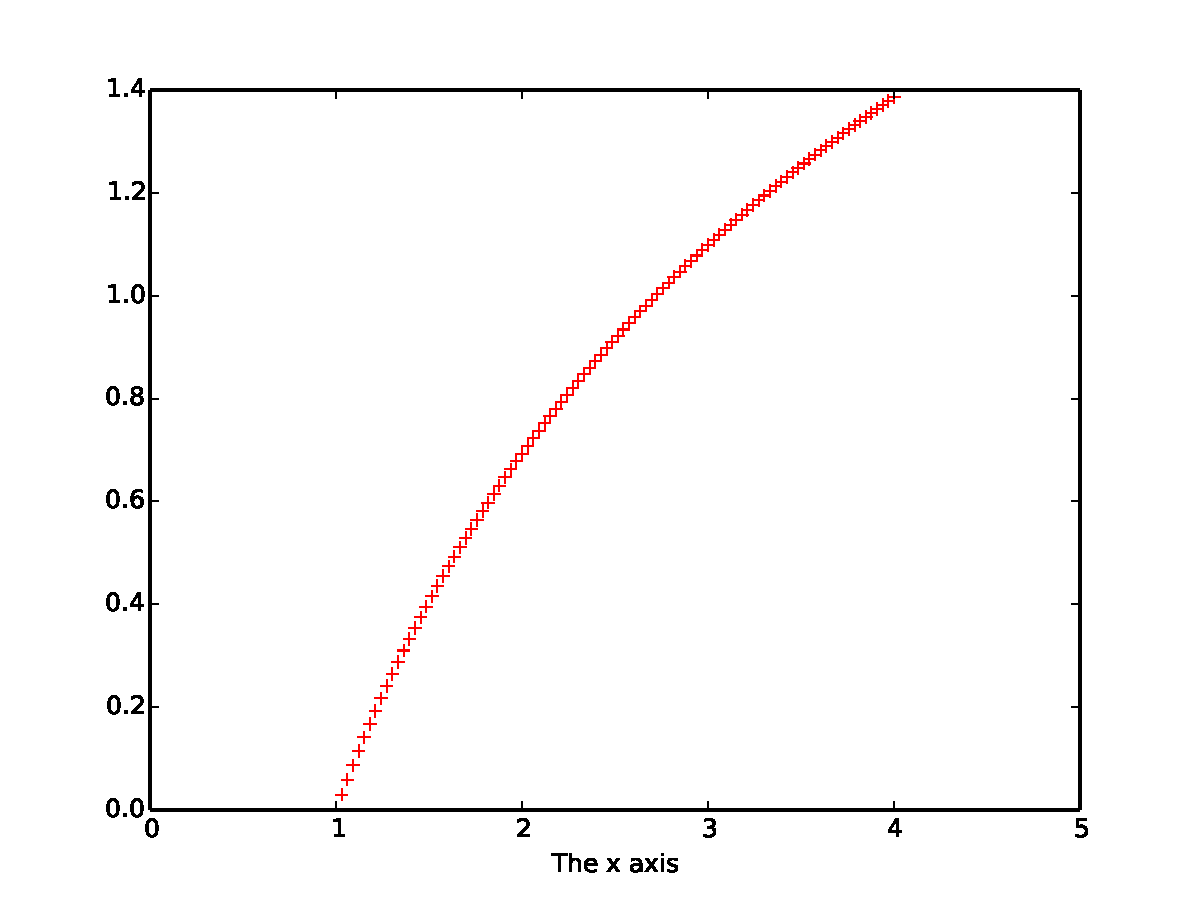
\includegraphics[width=\linewidth]{custom2.pdf}
    \label{fig:custom2}
\end{subfigure}
\label{fig:custom}
\end{figure}

See Appendix \ref{mpltables} for more comprehensive lists of colors, line styles, and figure customization routines.
    
\begin{problem} % Line plots with different domains but uniform style.
\label{prob:lineplot}
Write a function to plot the curve $f(x) = \frac{1}{x-1}$ on the domain $[-2,6]$.
Although $f(x)$ has a discontinuity at $x=1$, a single call to \li{plt.plot()} will attempt to make the curve look continuous.
\begin{enumerate}
\item Split up the domain and plot the two sides of the curve separately so that the graph looks discontinuous at $x=1$.
\item Plot both curves with a thick, dashed magenta line.\\
The keyword argument \li{linewidth} specifies the thickness of the line.
\item Change the range of the $y$-axis to be $[-6, 6]$.
\end{enumerate}
Your plot should look like the figure below.

\begin{figure}[H]
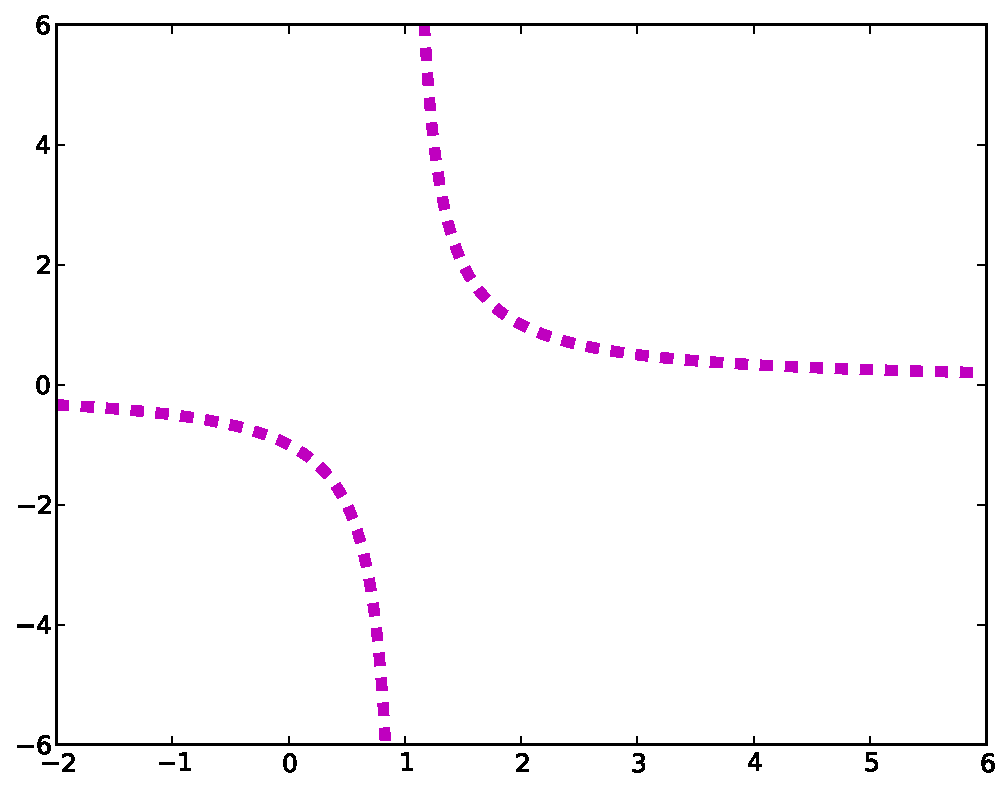
\includegraphics[width=.7\textwidth]{soln2.pdf}
\end{figure}
\end{problem}

\begin{comment} % Could still maybe be a good problem if simplified (?)
\begin{problem} Plot the curve $\frac{\sin(x)}{x+1}$ from $0$ to $10$.

Use blue shading under the curve when it is positive and red when it is negative (you may want to consider using \li{plt.fill_between()}.
Make the line dotted.
Label the x-axis ``x-axis'', the y-axis ``y-axis'',and the plot ``My Plot''.
Enable the grid lines.

Finally, use \li{plt.scatter()} to include a scatter plot of half of the value of the function at each of its maxima and minima in the range.
Display these points as upward-pointing triangles.
Don't forget to make sure the x limits of the plot are still 0 and 10.

\emph{Hint}: Since you are working with arrays of discrete values, you will want to find the index values where your $x$ and $y$ values are closest to the actual maxima and minima. As you work, consider the following:
\begin{itemize}
\item How would you manually find maxima and minima of a function?
\item How could you do something similar with your $x$ and $y$ arrays?
\end{itemize}
Your plot should look like the figure below.

\begin{figure}[H]
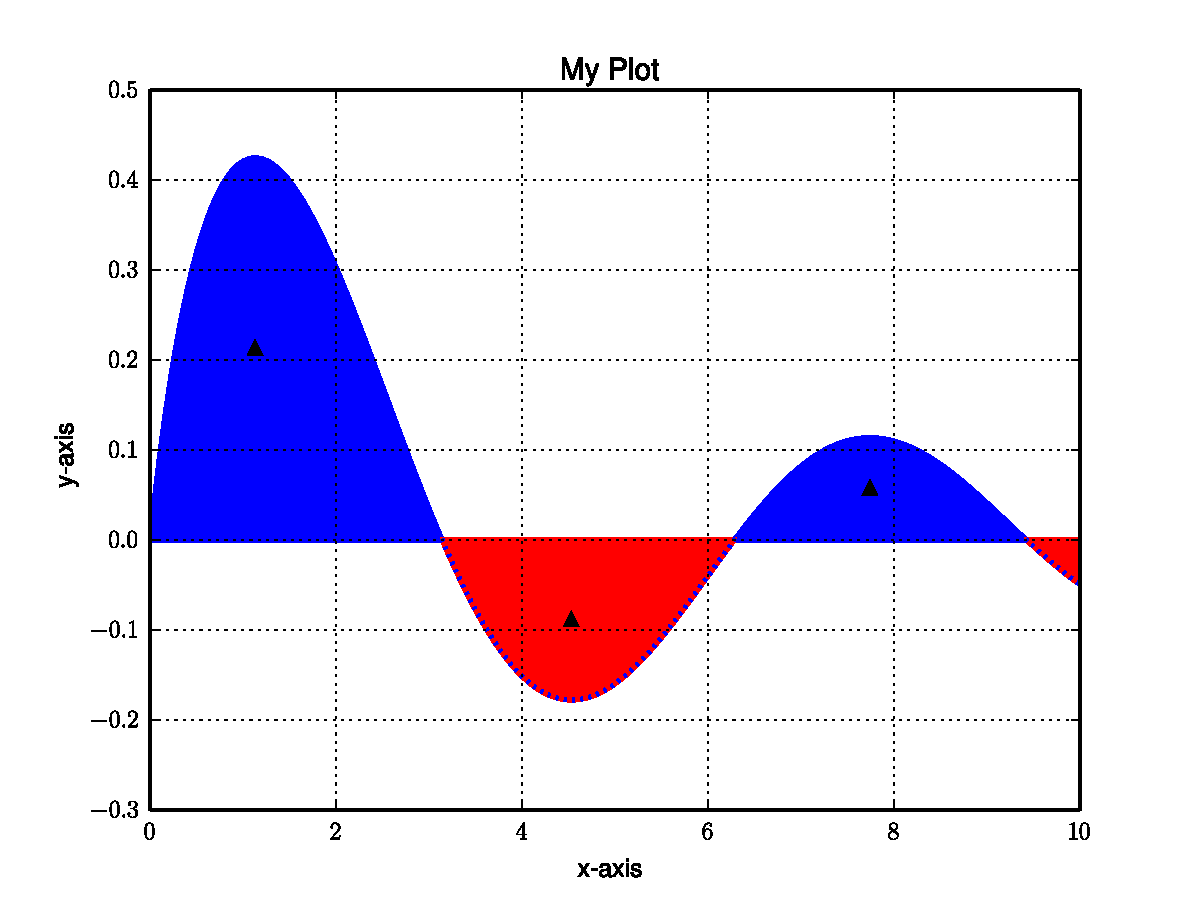
\includegraphics[width=\textwidth]{soln3.pdf}
\label{fig:problem3}
\end{figure}
\end{problem}
\end{comment}

\subsection*{Subplots} % ------------------------------------------------------

\emph{Subplots} are non-overlapping plots arranged in a grid within a single figure.
To create a figure with a grid of subplots, use \li{plt.subplot(numrows, numcols, fignum)}.
Here, \li{numrows} is the number of rows of subplots in the figure, \li{numcols} is the number of columns, and \li{fignum} specifies which subplot to modify.
% This index starts at 1 and increments across rows first.
See Figure \ref{fig:subplots}.

\begin{lstlisting}
>>> x = np.linspace(-np.pi, np.pi, 200)
>>> plt.subplot(2, 1, 1)            # Draw the first subplot.
>>> plt.plot(x, np.sin(x), 'b', linewidth=2)
>>> plt.xlim(-np.pi, np.pi)
>>> plt.subplot(2, 1, 2)            # Draw the second subplot.
>>> plt.plot(x, np.cos(x), 'c', linewidth=2)
>>> plt.xlim(-np.pi, np.pi)
>>> plt.show()                      # Show the figure with two subplots.
\end{lstlisting}

\begin{figure}[H] % Subplots
\captionsetup[subfigure]{justification=centering}
\centering
\begin{subfigure}{.49\textwidth}
    \centering
    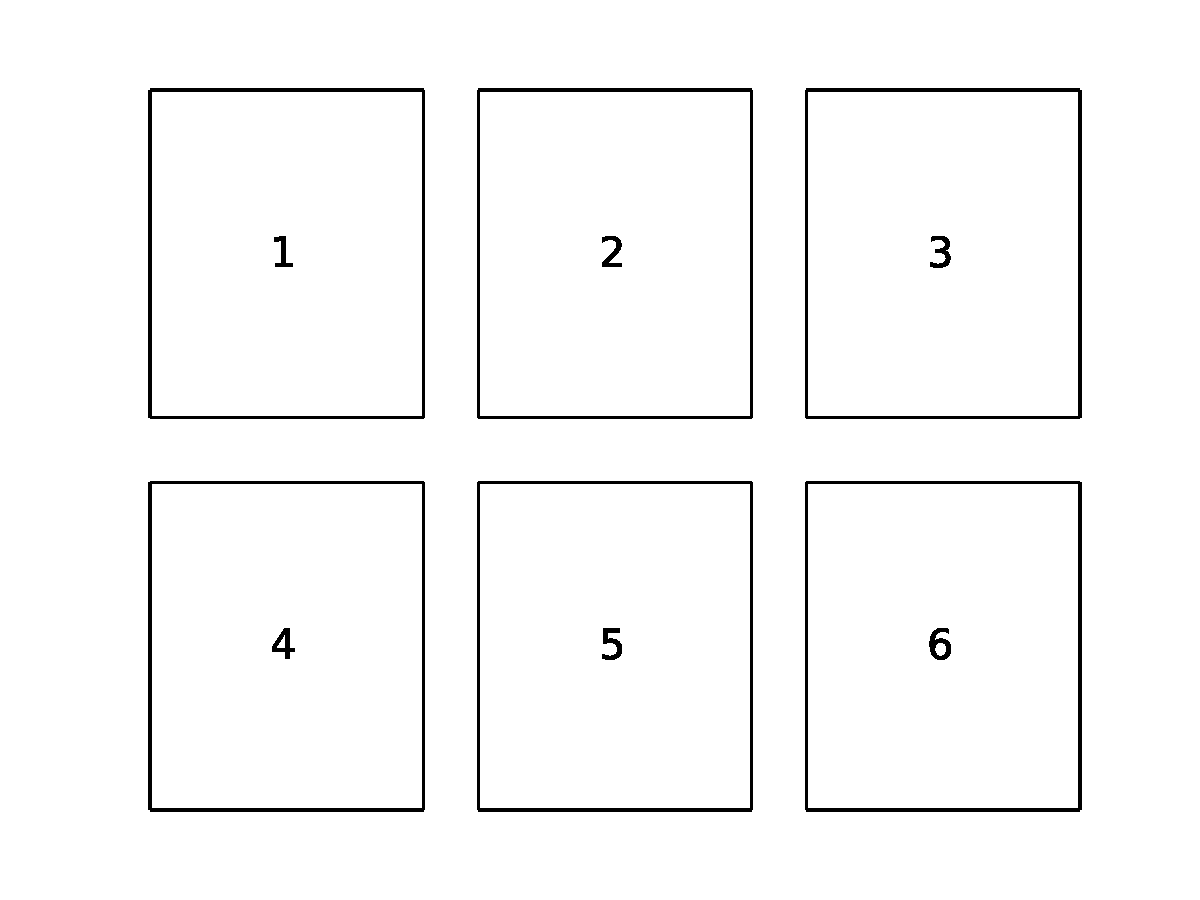
\includegraphics[width=\linewidth]{layout.pdf}
    \caption{The layout of subplots with \li{plt.subplot(2,3,i)} (2 rows, 3 columns), where \li{i} is the index pictured above.}
    \label{fig:layout}
\end{subfigure}
%
\begin{subfigure}{.49\textwidth}
    \centering
    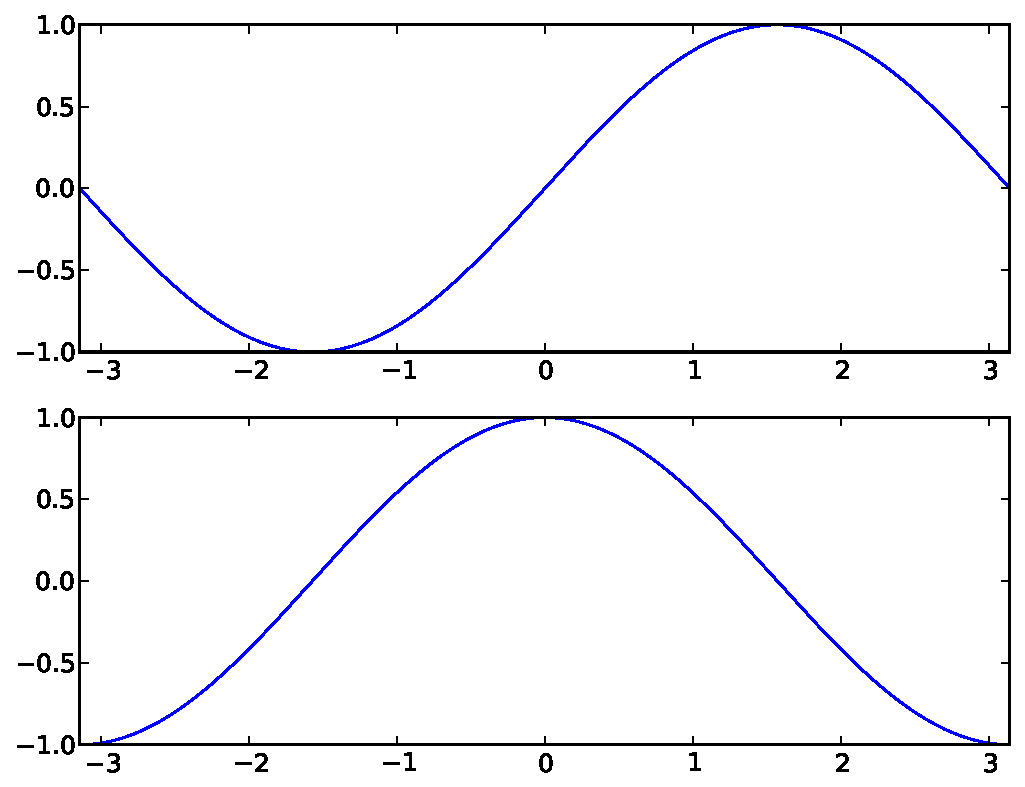
\includegraphics[width=\linewidth]{subplots.pdf}
    \caption{The graphs of $\sin(x)$ and $\cos(x)$ as subplots in a single figure with 2 rows\\and 1 column.}
    \label{fig:sincossubplots}
\end{subfigure}
\label{fig:subplots}
\end{figure}

\begin{problem} % Need a new subplots problem. Bernstein? (DataVis lab has it)
Make a plot with 4 subplots.
In the subplots place graphs of $e^x$, $sin(x)$, $cos(x)$, and $x^2$.
Plot each graph over the interval $(-\pi,\pi)$.
Title each graph accordingly and title the entire figure ``ALL THE PLOTS!"
\end{problem}

\section*{Other Kinds of Plots} % =============================================

% =============================================================================
% DONE TO HERE ================================================================
% =============================================================================

A \emph{histogram} is a way to visualize a 1-D data set, or list of values. 
A histogram is created by dividing up the range of the values into a finite number of intervals, or \emph{bins}.
Then, the number of values in each bin is added up.
Graphically, these totals are represented by bars whose length is equal to the number of values in the bin.

For example, suppose we randomly choose 20 integers between 1 and 10.
This code creates a histogram depicting how many of each number we chose.
Its output is in Figure \ref{fig:histogram}.

\begin{lstlisting}
x = np.random.randint(1, 11, 20)
plt.hist(x, bins=10, range=[.5, 10.5])
plt.show()
\end{lstlisting}

In this example our data set \li{x} consists of only integer values.
We created 10 bins in the range [.5, 10.5] so that each bin contains exactly one integer.

The function \li{plt.hist()} also returns some arrays, the first of which is a list of the total number of values in each bin.

We could also use a \emph{scatter plot} to visualize the random integers \li{x} that we generated in the previous example. 
The Matplotlib function call \li{plt.scatter(x,y)} draws a scatter plot from two 1-D arrays \li{x} and \li{y} by plotting the points \li{(x[i], y[i])}.
As an example, the code below produces Figure \ref{fig:scatter}.

\begin{lstlisting}
t = np.linspace(1,20,20)
# The argument 's' specifies the marker size.
plt.scatter(t, x, s=100)
plt.show()
\end{lstlisting}


\begin{figure}
\centering
\begin{subfigure}[t]{.49\textwidth}
\centering
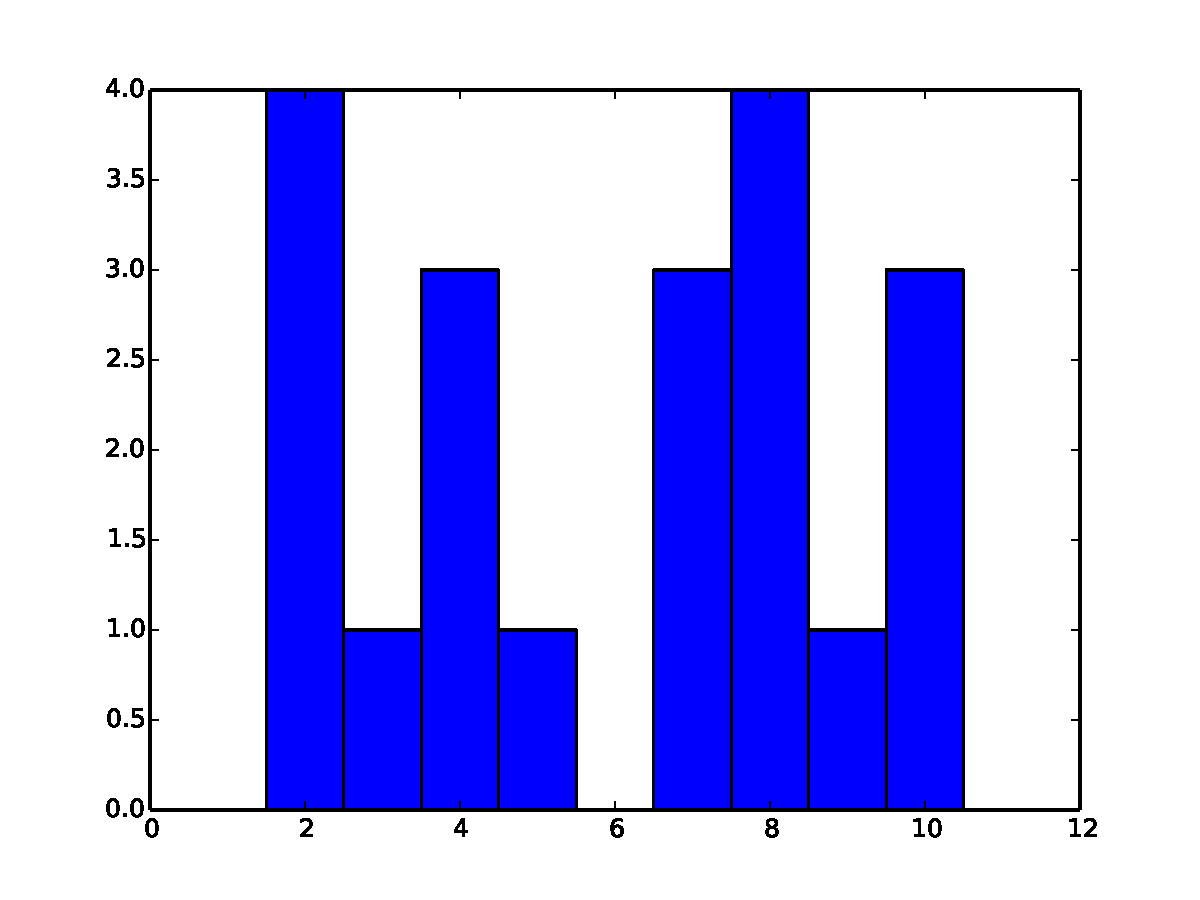
\includegraphics[width=\textwidth]{histogram.pdf}
\caption{A histogram.}
\label{fig:histogram}
\end{subfigure}
\begin{subfigure}[t]{.49\textwidth}
\centering
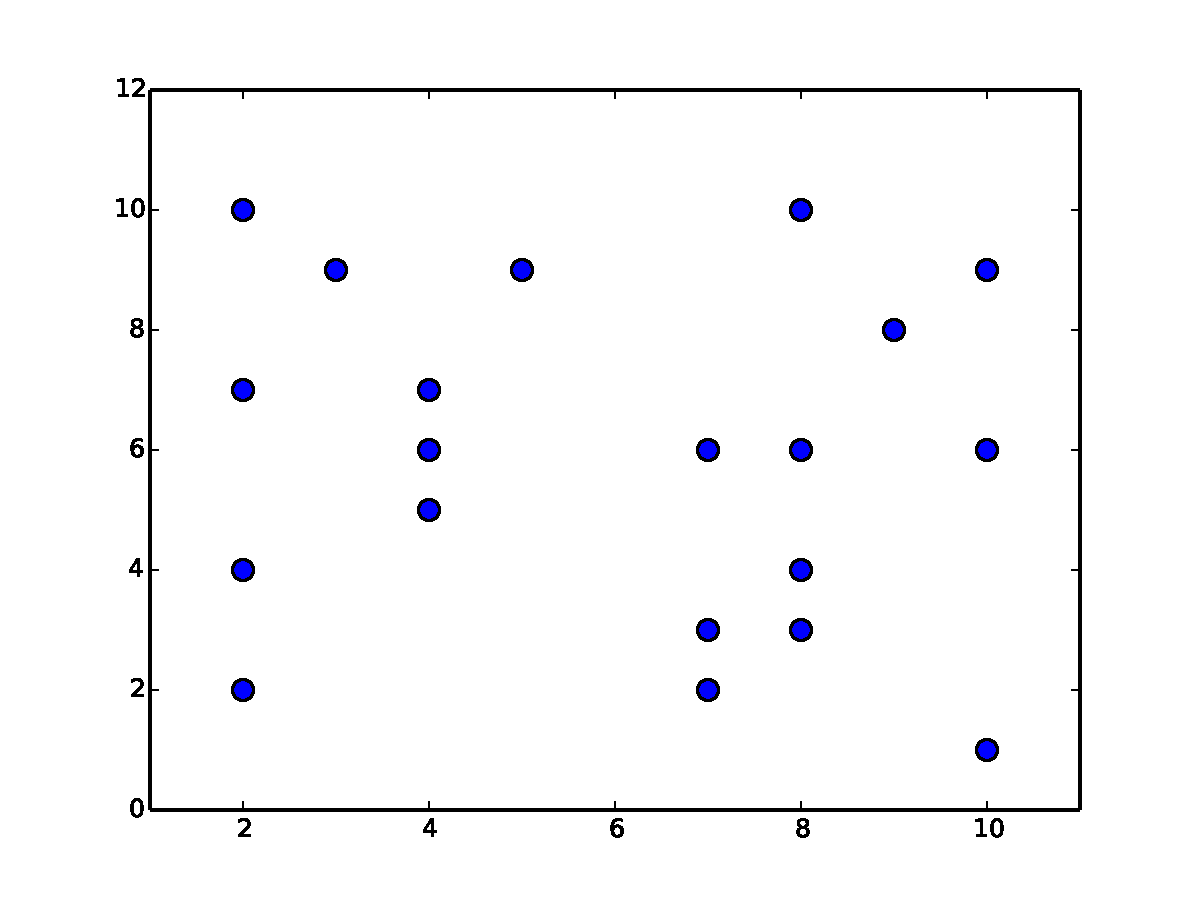
\includegraphics[width=\textwidth]{scatter.pdf}
\caption{A scatter plot.}
\label{fig:scatter}
\end{subfigure}

\caption{A histogram produced with \li{plt.hist()} and a scatter plot produced with \li{plt.scatter()}.}
\label{fig:otherplots}
\end{figure}

\begin{problem} % Find some real data to use with this problem. age v height?
\label{prob:subplot}
Write a function to generate the following plot:
\begin{enumerate}
\item Generate 50 random numbers in the interval $[0,1)$ with the function \li{np.random.rand()}.
\item Create a plot with two subplots. 
In the first subplot, draw a histogram of your data with 5 equally-sized bins.
\item In the second subplot, 
\begin{enumerate}
\item Draw a scatter plot of your data. 
Use the integers 1-50 for the $x$-coordinates and use your data for the $y$-coordinates.
\item Plot a red horizontal line whose height is equal to the mean of your data.
\end{enumerate}
\end{enumerate}

\begin{figure}[H]
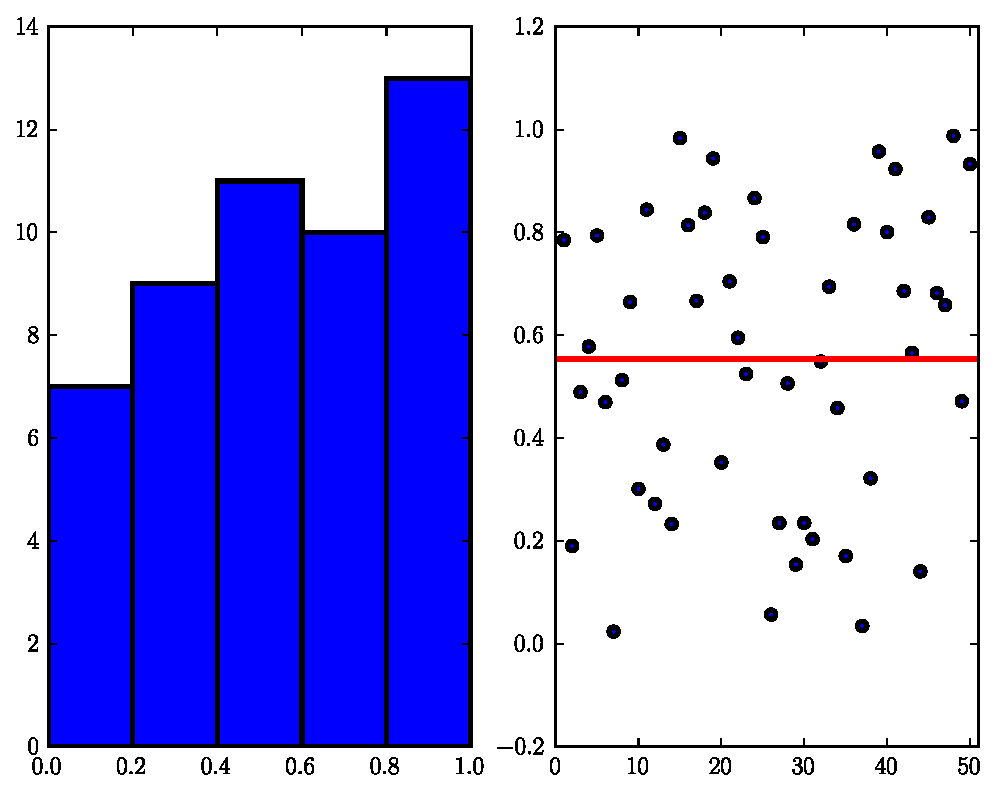
\includegraphics[width=.7\textwidth]{subplotProb.pdf}
% \caption{Correct output for Problem \ref{prob:subplot}.}
\label{fig:subplotProb}
\end{figure}
\end{problem}


\subsection*{Heatmaps} % ------------------------------------------------------

A function $f: \mathbb{R}^2 \rightarrow \mathbb{R}$ is usually plotted as a surface in $\mathbb{R}^3$.
A \emph{heatmap} visualizes such a function in only two dimensions by assigning the output of the function to a color (instead of a height).
For example, Figure \ref{fig:pcmexample} uses a heatmap to graph $f(x,y) = \sin(x)\sin(y)$ on $[-6,6] \times [-6,6]$.

The plot in Figure \ref{fig:pcmexample} was created with the function \li{plt.pcolormesh()}.
To draw Figure \ref{fig:pcmexample}, we must first create a grid of points at which to evaluate $f$.
We do this with the function \li{np.meshgrid()}, which is explained in Figure \ref{fig:meshgrid}.

\begin{figure}[H] % np.meshgrid() visual demonstration.
\begin{tikzpicture}[>=stealth', shorten <= .1cm,shorten >=.1cm, dot/.style=
    {circle,fill=black,minimum size=3pt,inner sep=0pt, outer sep=-1pt} ]

\foreach \x/\y in {0/0, 0/2, 0/4, 2/0, 2/2, 2/4, 4/0, 4/2, 4/4} 
    \node[draw, dot]at(\x,\y){};
\foreach \x/\y in {0/0, 0/1, 0/2, 1/0, 1/1, 1/2, 2/0, 2/1, 2/2} 
    \node[draw=none]at(\x*2-.5, \y*2+.3){(\x,\y)};

\foreach \x/\y in {0/0, 0/1, 0/2, 1/0, 1/1, 1/2, 2/0, 2/1, 2/2} 
    \node[draw=none]at(\x*.75+7, \y*.75+.1){\y};
\foreach \x/\y in {0/0, 0/1, 0/2, 1/0, 1/1, 1/2, 2/0, 2/1, 2/2} 
    \node[draw=none]at(\x*.75+7, \y*-.75+3.9){\x};

\draw[-, thick](6.7,-.25)--(6.7,1.95); 
\draw[-, thick](8.8,-.25)--(8.8,1.95);
\draw[-, thick](6.7,2.05)--(6.7,4.25);
\draw[-, thick](8.8,2.05)--(8.8,4.25);
\draw[-, thick](8.8,4.14)--(8.7,4.14);
\draw[-, thick](8.8,2.16)--(8.7,2.16);
\draw[-, thick](6.7,4.14)--(6.8,4.14);
\draw[-, thick](6.7,2.16)--(6.8,2.16);
\draw[-, thick](8.8,1.84)--(8.7,1.84);
\draw[-, thick](8.8,-.135)--(8.7,-.135);
\draw[-, thick](6.8,1.84)--(6.7,1.84);
\draw[-, thick](6.8,-.135)--(6.7,-.135);

\node[draw=none](X)at(6.3,.9){\texttt{Y}=};
\node[draw=none](y)at(6.3,3.15){\texttt{X}=};

\node[draw=none](point1)at(-.3, -.4){\texttt{x}=\big[0,};
\node[draw=none, node distance=2.35cm](point2)
    [right of=point1]{1,};
\node[draw=none, node distance=2cm](point3)
    [right of=point2]{2\big]};
\node[draw=none, rotate=270](point4)at(4.4,4.25)
    {\texttt{y}=\big[2,};
\node[draw=none, rotate=270, node distance=2.35cm](point5)
    [right of=point4]{1,};
\node[draw=none, rotate=270, node distance=2cm](point6)
    [right of=point5]{0\big]};
\end{tikzpicture}
\caption{This figure illustrates the function call \li{np.meshgrid(x, y)}, which returns the arrays \li{X} and \li{Y}. 
The returned arrays give the $x$- and $y$-coordinates of the points in the grid formed by \li{x} and \li{y}.}
\label{fig:meshgrid}
\end{figure}

\begin{lstlisting}
# Create an XY meshgrid
x = np.linspace(-6, 6, 401)
y = np.linspace(-6, 6, 401)
X, Y = np.meshgrid(x, y)
\end{lstlisting}
The arrays $X$ and $Y$ satisfy \li{(X[i,j], Y[i,j]) = (x[i],y[j])}.

Now we can evaluate $f(x,y)$ at each point in the grid and plot the result.

\begin{lstlisting}
f = np.sin(X) * np.sin(Y)
plt.pcolormesh(X, Y, f)
plt.colorbar()    # Show scale
plt.show()
\end{lstlisting}
This plot is shown in Figure \ref{fig:pcmexample}

\begin{figure} % 2D heat map
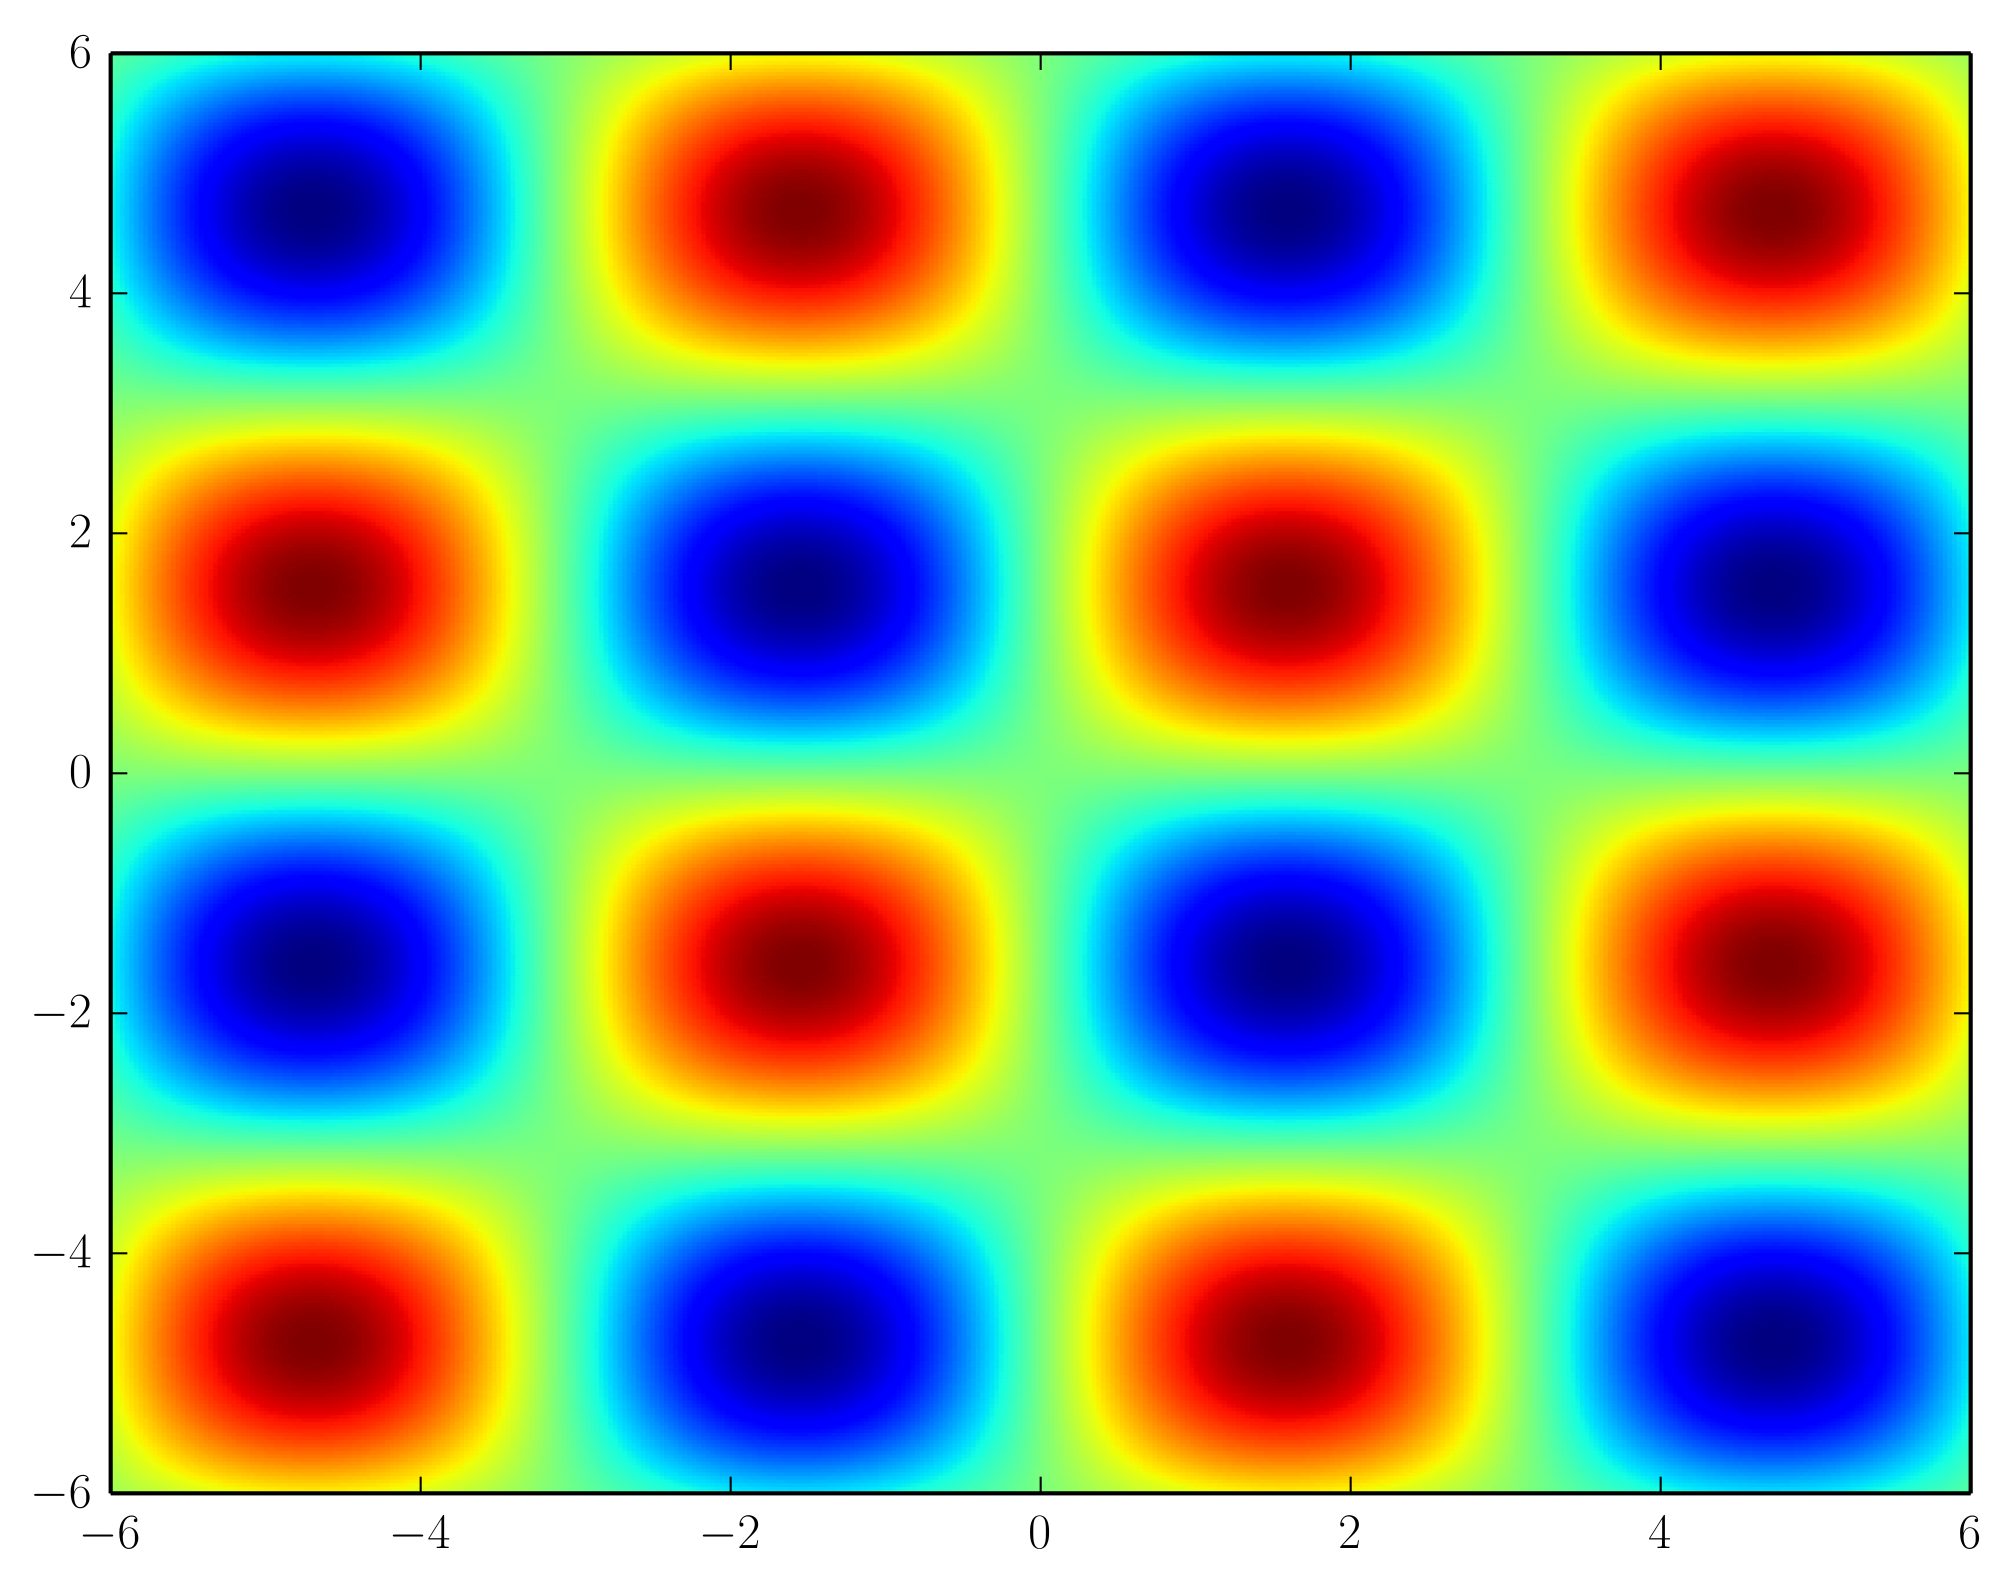
\includegraphics[width=.7\textwidth]{sinxsiny.png}
\caption{A heatmap of $f(x,y)=\sin\left(x\right)\times\sin\left(y\right)$ drawn by \li{plt.pcolormesh()}.}
\label{fig:pcmexample}
\end{figure}


\begin{problem} % Heatmap problem
\label{prob:heatmap}
\leavevmode
\begin{enumerate}
\item Plot the function $f(x,y) = \frac{\sin(x)\sin(y)}{xy}$ on $[-2\pi,2\pi] \times [-2\pi,2\pi]$. 
Include the scale bar in your plot.
\item Change the color scheme of your plot with the keyword argument \li{cmap='seismic'} in the call to \li{plt.pcolormesh()}. 
You can see a list of all possible color schemes at \url{http://matplotlib.org/examples/color/colormaps_reference.html}.
\item Change the limits on the $x$- and $y$-axes so that the plot is only over the domain $[-2\pi,2\pi] \times [-2\pi,2\pi]$.
\item Fix the aspect ratio of your plot so that it is a square using the line \li{plt.gca().set_aspect('equal')}.
\end{enumerate}
Your finished plot should look like Figure below.

\begin{figure}[H]
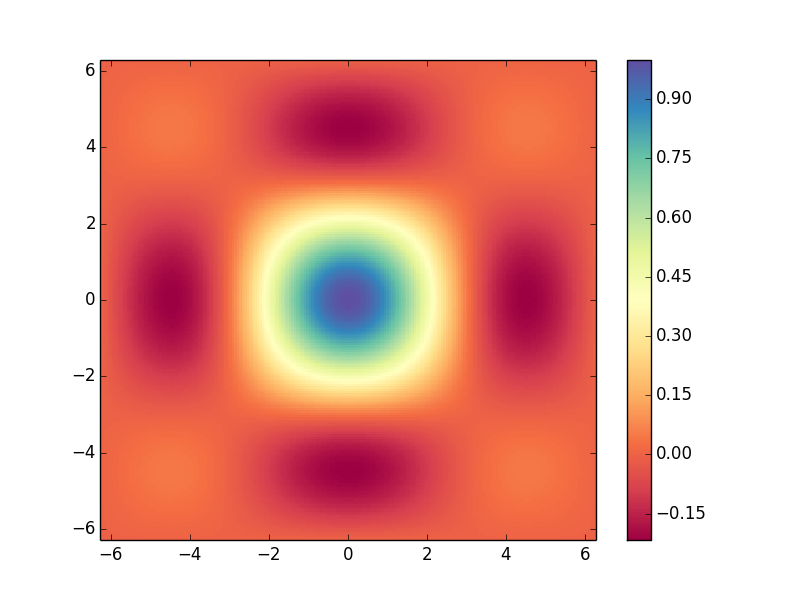
\includegraphics[width=.7\textwidth]{pcolor2.png}
% \caption{Correct output for Problem \ref{prob:heatmap}.}
% \label{fig:heatmapProb}
\end{figure}
\end{problem}

\begin{comment}
\begin{table} % Different plotting commands. Might be useful to put this back in.
\centering
\begin{tabular}{|l|p{7cm}|p{3cm}|}
    \hline
    Function & Description & Usage\\
    \hline
    \li{bar} & makes a bar graph & bar(left,height)\\
    \li{barh} & makes a horizontal bar graph & barh(bottom,width)\\
    \li{fill} & plots lines with shading under the curve & fill(x,y)\\
    \li{fill\_between} & plots lines with shading between two given y
    values & fill\_ between(x,y1, y2=0)\\
    \li{hist} & plots a histogram from data & hist(data)\\
    \li{pie} & makes a pie chart & pie(x)\\
    \li{plot} & plots lines and data on standard axes & plot(x,y)\\
    \li{polar} & plots lines and data on polar axes & polar(theta,r)\\
    \li{loglog} & plots lines and data on logarithmic x and y axes &
    loglog(x,y)\\
    \li{scatter} & plots data, has more options for scatter plots than
    the plot function & scatter(x,y)\\
    \li{semilogx} & plots lines and data with a log scaled x axis &
    semilogx(x,y)\\
    \li{semilogy} & plots lines and data with a log scaled y axis &
    semilogy(x,y)\\
    \li{specgram} & makes a spectogram from data & specgram(x)\\
    \li{spy} & plots the sparsity pattern of a 2D array & spy(Z)\\
    \li{triplot} & plots triangulation between given points &
    triplot(x,y)\\
\end{tabular}
\end{center}
\caption{Some basic functions in Matplotlib.}
\label{mpl:basics}
\end{table}
\end{comment}

\begin{comment} % 3D plotting with Matplotlib (shorten and reinsert)
Matplotlib can also be used for 3D plotting. The following is an example
of how to use Matplotlib to plot the function $z=\sin(x)\sin(y)$ with
both x and y ranging from -6 to 6. The resulting plot is shown in Figure
\ref{mpl:3dplot}. If you change the number of sample points used you
will notice that graphs look much nicer with large numbers of sample
points, but it will also take much longer for your computer to render
the image.

\begin{lstlisting} 
from mpl_toolkits.mplot3d import Axes3D 
from matplotlib import pyplot as plt 
import numpy as np 
fig = plt.figure() 
ax= fig.gca(projection='3d') 
x = np.linspace(-6, 6, 301) 
y = np.linspace(-6, 6, 301) 
X, Y = np.meshgrid(x, y) 
Z = np.sin(X) * np.sin(Y) 
ax.plot_surface(X, Y, Z) 
plt.show() 
\end{lstlisting}

\begin{figure} 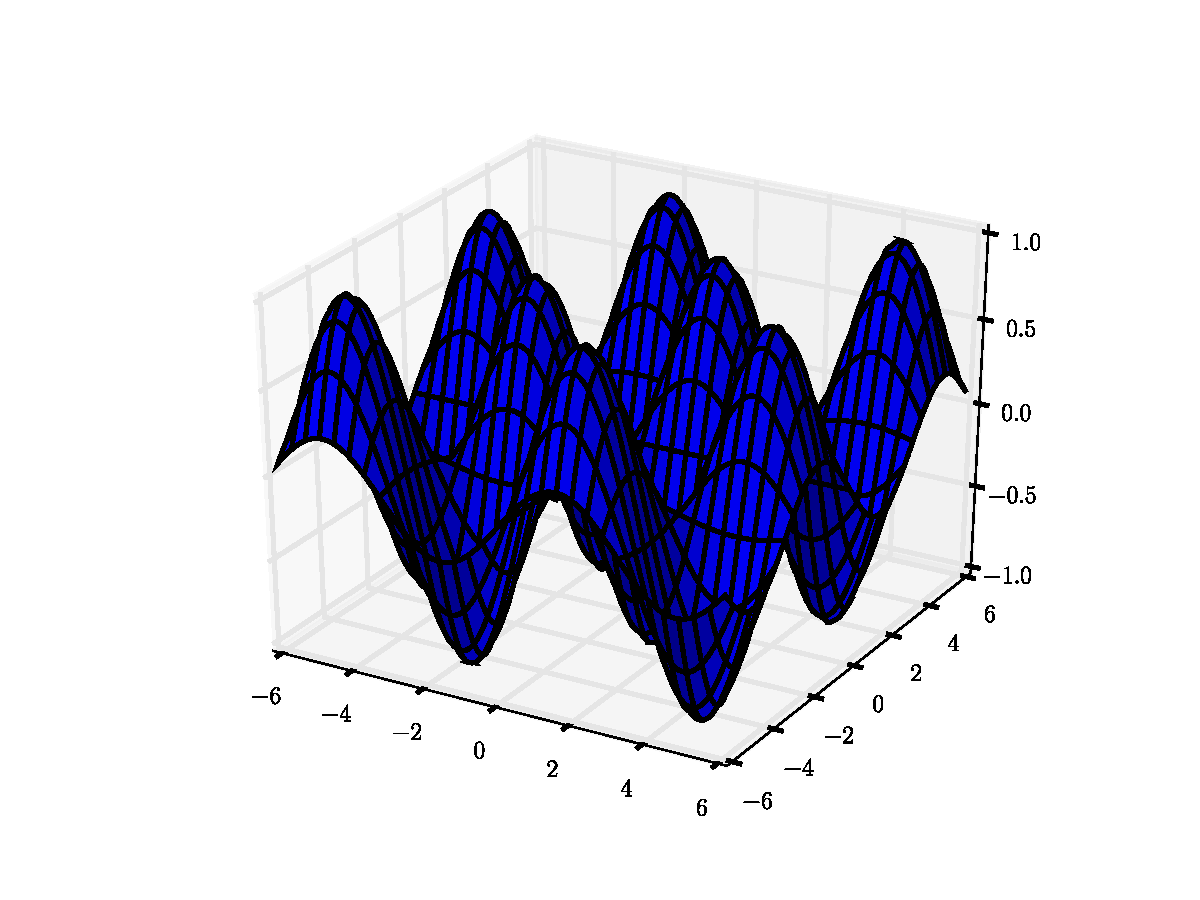
\includegraphics[width=\textwidth]{3dplot.pdf} \caption{A
3D plot of $\sin\left(x\right)\times\sin\left(y\right)$.}
\label{mpl:3dplot} \end{figure}

\begin{problem} Plot the function \begin{equation*}
\frac{\cos\left(\sqrt{x^2 + y^2}\right)}{\frac{x^2 + y^2}{10} + 1}
\end{equation*} on $[-10, 10] \times [-10, 10]$. \end{problem}
\end{comment}

\section*{3-D plotting with Mayavi}

Although Matplotlib is capable of creating 3-D plots, Mayavi does it much faster and with better visuals. 
We will use Mayavi for all 3-D plots in these labs. % O RLY?
For information beyond what is found in this tutorial, see \url{http://docs.enthought.com/mayavi/mayavi/}.
To get started, import \li{mlab} from \li{mayavi}.

\begin{lstlisting}
from mayavi import mlab
\end{lstlisting}

\begin{info} % Installation note. Make into a footnote?
If you do not have the \li{Mayavi} package installed on your system, you may download it by running the following commands from the command line:
\begin{lstlisting}
$ conda install conda               # Download the most recent installer.
$ conda install anaconda            # Update all packages.
$ conda install mayavi              # Installs mayavi.
\end{lstlisting}

For more information regarding installing Python packages, see Appendix \ref{updateinstall}.
\end{info}
%$

The module \li{mlab} has many plotting functions.
We will introduce a few in this lab; for more see \url{http://docs.enthought.com/mayavi/mayavi/auto/mlab_helper_functions.html}.
You can also browse examples at \url{http://docs.enthought.com/mayavi/mayavi/auto/examples.html}.

\begin{comment}
\begin{table} % Mayavi plotting functions. Probably should put this back in.
\begin{center}
\begin{tabular}
{|c|l|}
\hline
Function & Description \\
\hline
\li{barchart} & Produces 3D histogram-like plots\\
\li{contour3d} & Plots level surfaces of functions of three variables\\
\li{flow} & Creates a trajectory of particles following the flow of a vector field\\
\li{imshow} & Use a colormap to view a 2D array as an image\\
\li{mesh} & Plot a surface using \li{(x,y,z)} coordinates supplied as three 2D arrays\\
\li{plot3d} & Draws lines between points\\
\li{points3d} & Plots glyphs (like points) at the coordinates supplied\\
\li{quiver3d} & Generate 3D vector fields\\
\li{surf} & Plot a surface with a 2D array as elevation data\\
\hline
\end{tabular}
\end{center}
\caption{Some plotting functions in \li{mlab}.}
\label{table:mlab_functions}
\end{table}
\end{comment}

\begin{comment}
All these functions can be ``tested" (which provides an example figure for the function) with the command:
\begin{lstlisting}
mlab.test_<plotting function>()
mlab.show()
\end{lstlisting}
Note that pressing tab after typing \li{mlab.test_} will provide a list of available commands and that, like Matplotlib, we use the \li{show()} command to actually view our plot.

For example, to test the \li{fancy_mesh()} function, we run the following:
\begin{lstlisting}
mlab.test_fancy_mesh()
mlab.show()
\end{lstlisting}

The result should resemble Figure \ref{fig:fancymesh}.

\begin{figure}
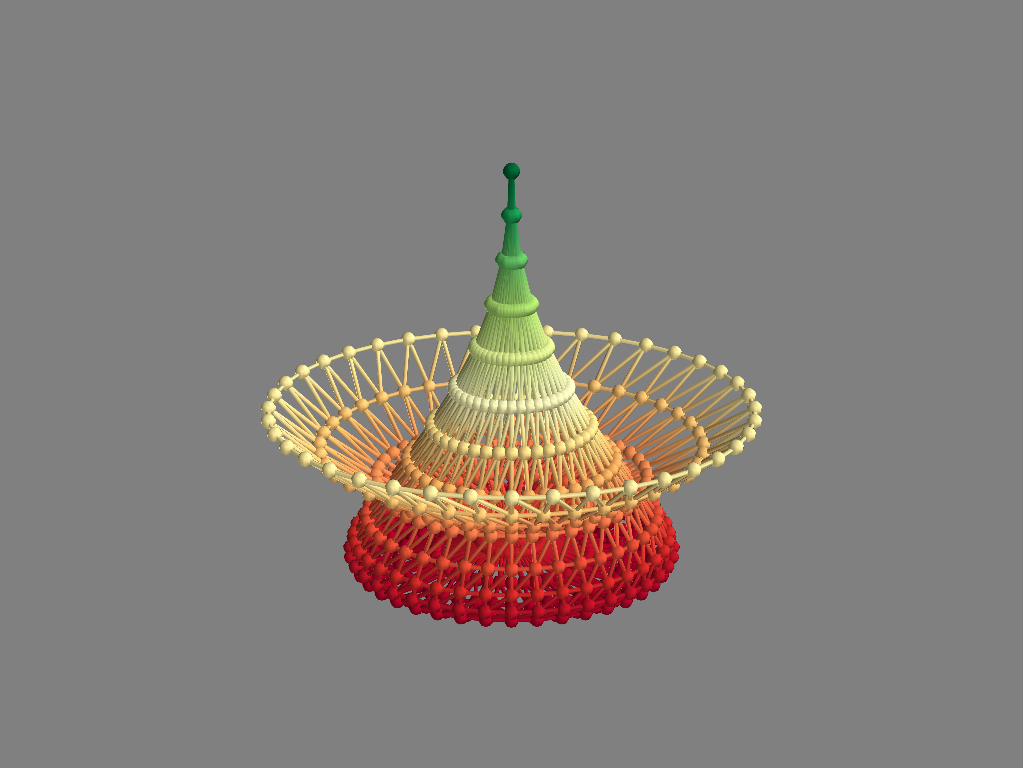
\includegraphics[width=\textwidth]{fancymesh.png}
\caption{An example of the fancy mesh plotting function}
\label{fig:fancymesh}
\end{figure}

In this lab, we will focus our attention on introducing the \li{mesh}, \li{plot3d}, and \li{points3d} functions.

Like matplotlib, \li{mlab} takes a set of data points and plots it.
However, instead of passing just \li{x} and \li{y} coordinates as we did in Matplotlib, we also send \li{z} coordinates to produce a 3D plot.
\end{comment}

\subsection*{Lines} % ---------------------------------------------------------

The function call \li{mlab.plot3d(x,y,z)} plots the points \li{(x[i], y[i], z[i])} and connects them with straight lines.
The code below produces the flower in Figure \ref{fig:plot3d}

\begin{lstlisting}
num = np.pi/1000
pts = np.arange(0, 2*np.pi + num, num)
x = np.cos(pts) * (1 + np.cos(pts*6))
y = np.sin(pts) * (1 + np.cos(pts*6))
z = np.sin(pts*6/11)
mlab.plot3d(x, y, z)
mlab.show()
\end{lstlisting}

% TODO: merge this figure with the mlab.points3d() figure.
\begin{figure}
\captionsetup[subfigure]{justification=centering}
\centering
\begin{subfigure}{.5\textwidth}
    \centering
    
\includegraphics[width=\linewidth]{plot3d.png}
    \caption{Sample output of \li{mlab.plot3d()}.}
    \label{fig:plot3d}
\end{subfigure}%
\begin{subfigure}{.5\textwidth}
    \centering
    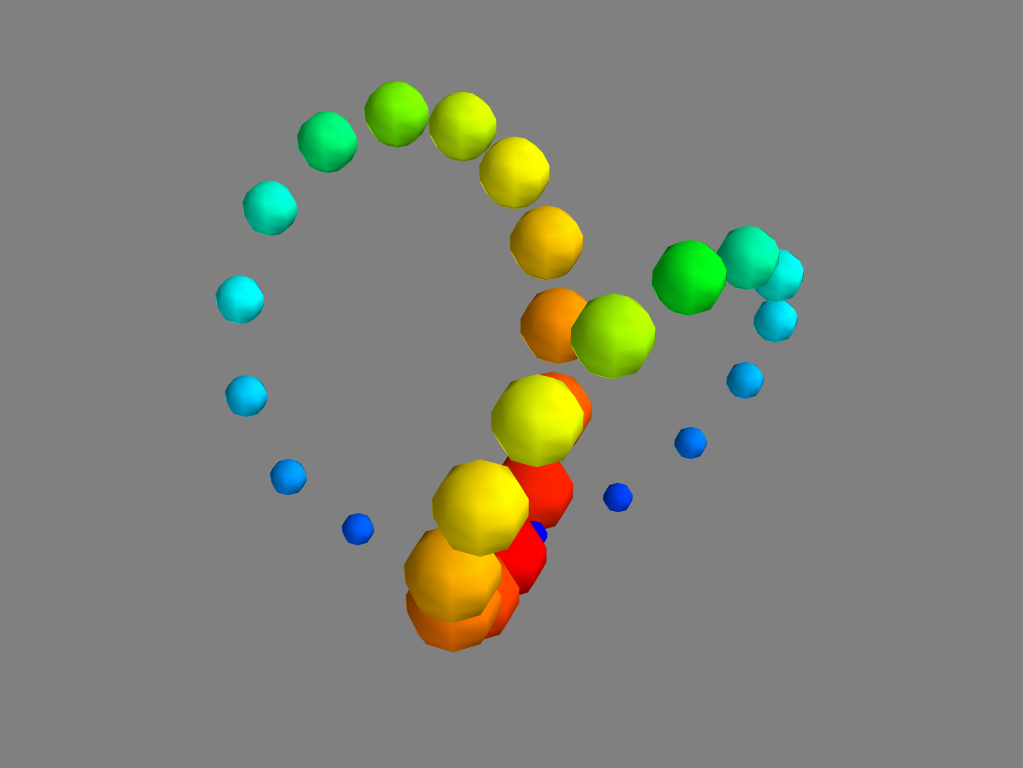
\includegraphics[width=\linewidth]{points3d.png}
    \caption{Sample output of \li{mlab.points3d()}.}
    \label{fig:points3d}
\end{subfigure}
\end{figure}

\subsection*{Points} % --------------------------------------------------------

The function call \li{mlab.points3d(x,y,z)} plots the points \li{(x[i], y[i], z[i])}, but does not connect them. 
In the code below, the optional input array \li{s} defines a scalar for each point that modifies the color and size of the point.
The output is in Figure \ref{fig:points3d}.

\begin{lstlisting}
pts = np.linspace(0, 4 * np.pi, 30)
x = np.sin(2 * pts)
y = np.cos(pts)
z = np.cos(2 * pts)
s = 2+np.sin(pts)
# Adjust the keyword argument 'scale_factor' so all points are visible.
mlab.points3d(x, y, z, s, scale_factor=.15)
mlab.show()
\end{lstlisting}

\subsection*{Surfaces} % ------------------------------------------------------

You can draw a surface in mayavi with \li{mlab.surf()}.
This function accepts three arrays, \li{X}, \li{Y}, and \li{Z}, where \li{X} and \li{Y} determine a grid of points similar to the output of \li{np.meshgrid()}.
The array \li{Z} gives the height of the surface at each of these points.

The output of \li{np.meshgrid()} is the transpose of what \li{mlab.surf()} expects.
To avoid confusion, use the function \li{np.mgrid()} instead.
This function uses the slicing syntax \li{[start:stop:step]} 
The code below produces the hyperbolic paraboloid in Figure \ref{fig:surf_example}.

\begin{lstlisting}
X, Y = np.mgrid[-4:4:0.025, -4:4:0.025]
Z = X**2/4-Y**2/4
mlab.surf(X, Y, Z, colormap='RdYlGn')
mlab.show()
\end{lstlisting}

\begin{figure}
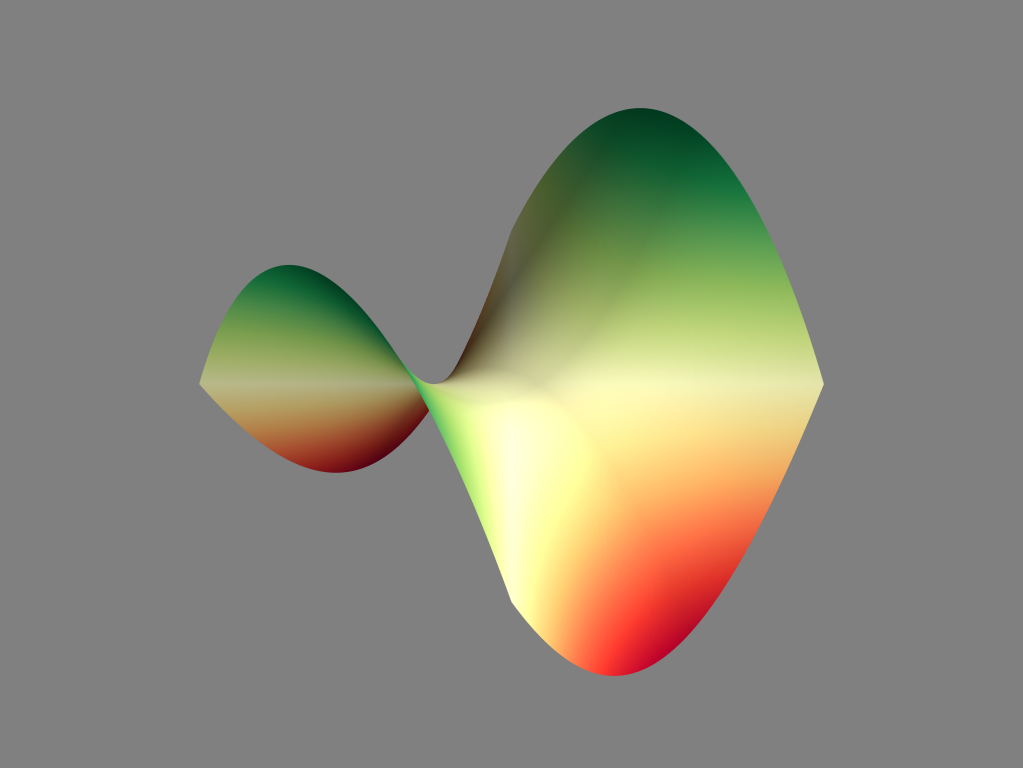
\includegraphics[width=.7\textwidth]{mesh_example.png}
\caption{Sample output of \li{mlab.surf()}.}
\label{fig:surf_example}
\end{figure}

The plotting functions in Mayavi allow you to specify the color of a plot, either as a solid color or with a varying colormap.
For example, the plot in Figure \ref{fig:surf_example} uses the colormap \li{'RdYlGn'}.
For a list of all colormaps in Mayavi, see \url{http://docs.enthought.com/mayavi/mayavi/mlab_changing_object_looks.html}.

\begin{problem}
Plot the function $z = \frac{1}{10}\sin(10(x^2+y^2))$ on $[-1,1] \times [-1,1]$ using Mayavi.
\end{problem}

%TODO: this problem is copied from https://github.com/enthought/mayavi/blob/master/examples/mayavi/mlab/canyon.py.
% we either need to cite this (and thus give the solution) or find a different problem.
\begin{comment}
\begin{problem}
\label{prob:grand_canyon}
Provided Grand Canyon topological radar data from NASA, do the following.

\begin{itemize}
\item Reshape the data to be 3601x3601.
\item Cast the data type as \li{float32}.
\item Slice the data, taking the first 1000 rows and columns 900-1900.
\item There is some missing data, so set the minimum of your data equal to the minimum of the the positive data points.
\item Preset the figure using the following commands: \li{mlab.figure(size=(400,320)}, \li{bgcolor = (.16, .28, .46))}
\item Now plot with \li{mlab.surf}, using the colormap \li{gist_earth}, with a \li{warp_scale=.2}, \li{vmin=1200}, and \li{vmax=1610}.
\item Take a smaller view of the canyon using \li{mlab.view(-5.9, 83, 570, [5.3, 20, 238])}.
\end{itemize}

This should produce Figure \ref{fig:GrandCanyon}

\begin{figure}[H]
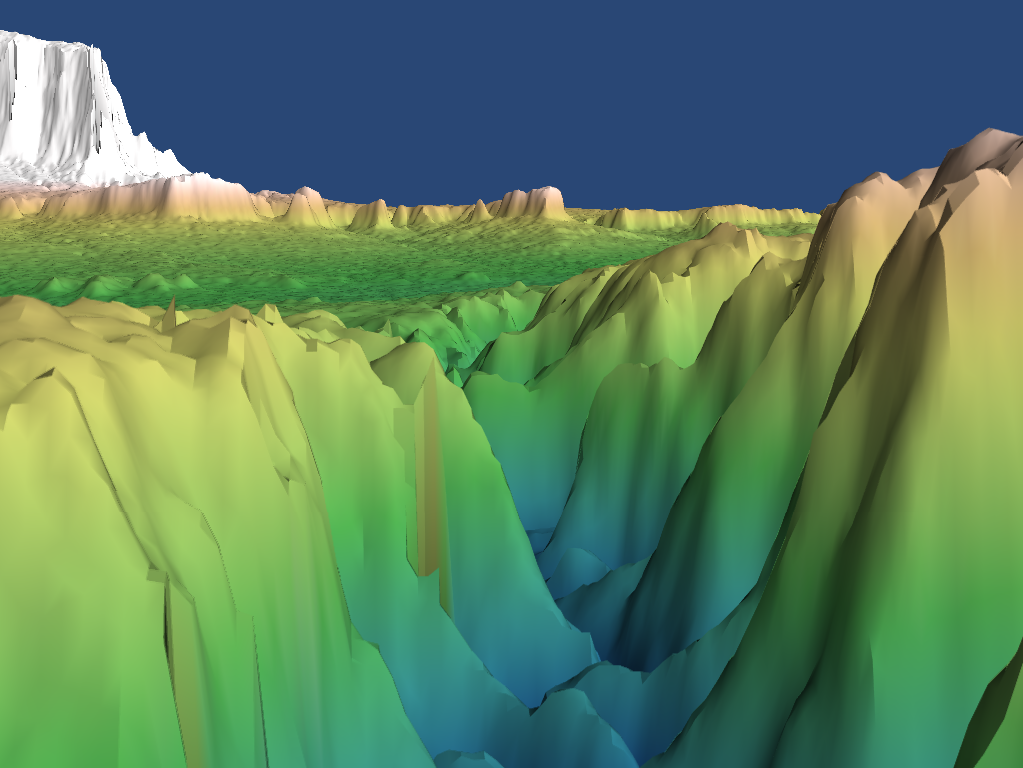
\includegraphics[width=.7\textwidth]{GrandCanyon.png}
\caption{Correct output for Problem \ref{prob:grand_canyon}.}
\label{fig:GrandCanyon}
\end{figure}

\end{problem}
\end{comment}

\section*{References}

See \url{http://matplotlib.org} for Matplotlib documentation.

\newpage

\section*{Additional Material} % ==============================================


% =============================================================================
% =============================================================================
% Stuff to move ===============================================================
% =============================================================================
% =============================================================================

\begin{comment}
\begin{info} % IPython Notebook inline plotting (move to another lab!)
If you are executing these Matplotlib commands in an IPython shell, executing the \li{plt.show} method will open a new window with the plot. If you are using IPython Notebook, you have the option to display the plots within your notebook. You may opt into this feature by running \li{\%matplotlib inline} or \li{\%matplotlib notebook} in your IPython Notebook. The \li{inline} option shows the plot, whereas the \li{notebook} option shows the plot and provides controls to interact with the plot. Additionally, when using this option, the plot is displayed after running the \li{plt.plot} command; the \li{plt.show} command is not necessary. 
\end{info}
\end{comment}

\begin{comment} % Interactive graphs with widgets. Additional Info?
Matplotlib also allows us to make interactive graphs as follows:

% This example is largely based on one of the examples in the Matplotlib
% docs. I have simplified it and changed the way the libraries are
% imported, but we could do a citation anyway.
%
\begin{lstlisting} 
import numpy as np 
from matplotlib import pyplot as plt 
from matplotlib import widgets as wg 
ax = plt.subplot(111)
plt.subplots_adjust(bottom=.25) 
t = np.arange(0., 1., .001) 
a0 = 5. 
f0 = 3. 
s = a0 * np.sin(2 * np.pi * f0 * t) 
l = plt.plot(t, s)[0]
plt.axis([0, 1, -10, 10]) 
axfreq = plt.axes([.25, .05, .65, .03]) 
axamp = plt.axes([.25, .1, .65, .03]) 
sfreq = wg.Slider(axfreq, 'Freq', .1, 30., valinit=f0) 
samp = wg.Slider(axamp, 'Amp', .1, 10., valinit=a0) 
def update(val): 
    amp = samp.val 
    freq = sfreq.val 
    l.set_ydata(amp * np.sin(2 * np.pi * freq * t)) 
    plt.draw() 
sfreq.on_changed(update)
samp.on_changed(update) 
plt.show() 
\end{lstlisting} The resulting plot is shown in Figure \ref{mpl:interact}.

\begin{figure} 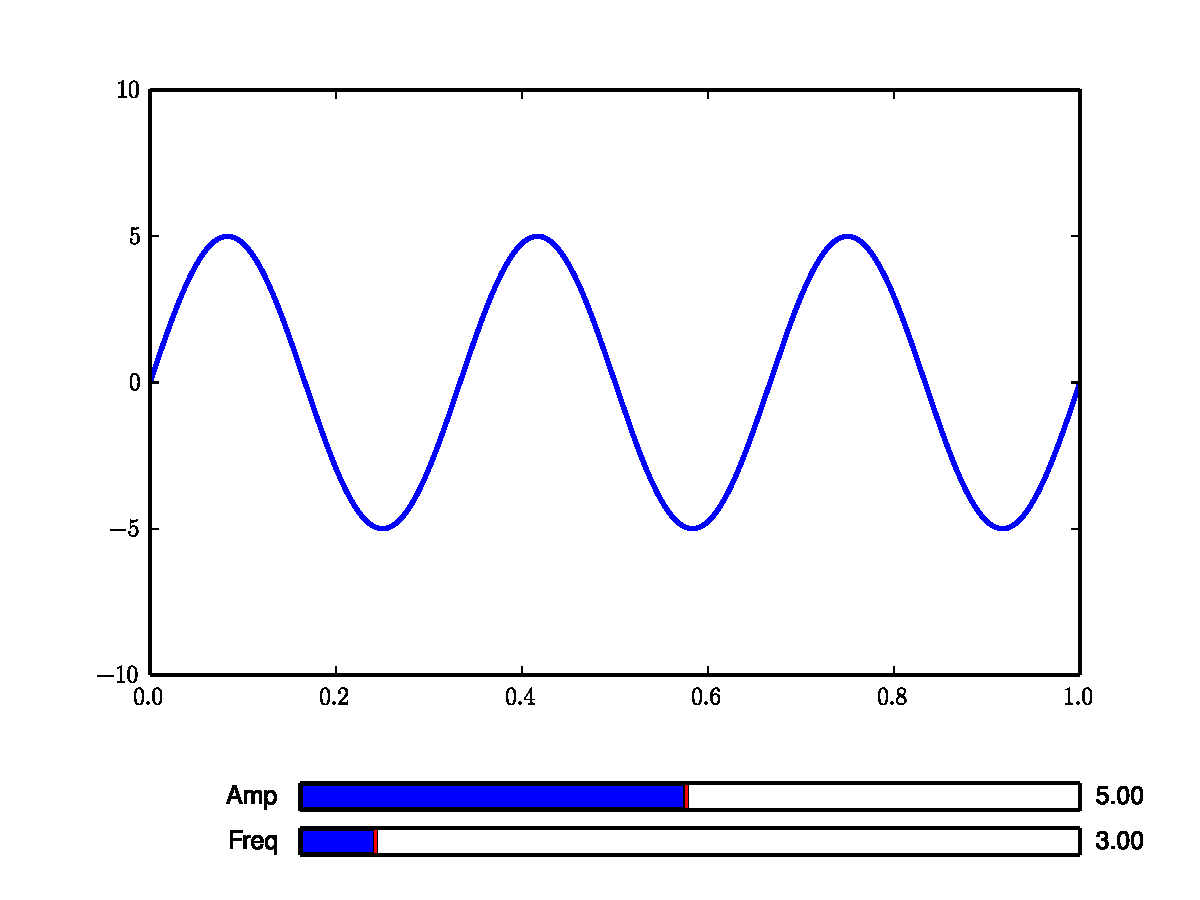
\includegraphics[width=\textwidth]{interact.pdf}
\caption{A snapshot of an interactive plot made using Matplotlib.}
\label{mpl:interact} \end{figure}

\begin{problem} Modify the code above to add a third slider to
manipulate the phase of the wave shown. Have it range from 0 to $2\pi$
and set the default value to zero. \end{problem}

\end{comment}

\begin{comment} % This will be covered in the Complex labs.
\begin{problem} Use \li{plt.pcolormesh()} to plot the absolute value of the function $x^3 +2x^2 -x +3$ on the complex plane with 0 $\leq$ \li{x} $\leq$ 2 and 0 $\leq$ \li{y} $\leq$ 2.
\emph{Helpful Hint}: First create your domain arrays, then convert these to a single array of complex variables to evaluate the function.

Your plot should look like Figure \ref{fig:pcolormesh}.

\begin{figure}[H] % Complex colorplot
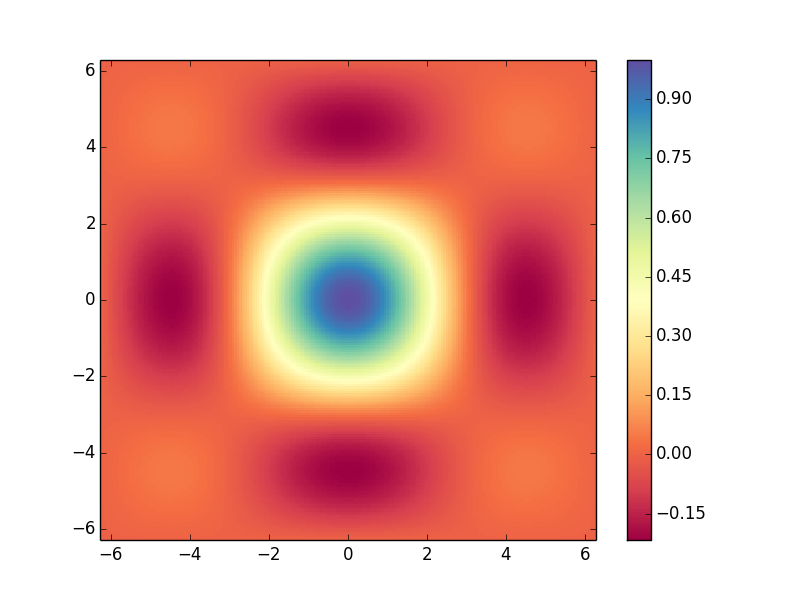
\includegraphics[width=\textwidth]{pcolor2.png}
\caption{Another example of a colorplot.}
\label{fig:pcolormesh}
\end{figure}
\end{problem}
\end{comment}
